\section*{Introduction}

In his video essay, A Future of Medicine, Dr. Bernard postulates on a world that views our current system of evidence based medicine, as we see European plague doctors. Because in our modern system of evidence based medicine, we extrapolate population data to a given person, for the purpose of predicting outcome. Which you may ask, what is the problem with such? 

To explain, from a practical standpoint, consider this. What if, instead of running a trial on thousands of disperse persons. What if you were simply cloned, hundreds of thousands of times, and therein, we performed hundreds of thousands of trials, forming a stochastic model that likewise predicts outcome for some given treatment?

As Dr. Bernard points out, if a trial was done on a bunch of men, there have been documented cases where women taking the very same medication experienced different reactions. Nowadays, trials are required to include notable age, gender, and race/ethnicity demographics. But as Kravitz pointed out, ``[this] may do nothing but ensure that the estimates for any one subgroup are unreliable due to small numbers''. In the very same paper, Kravitz coined this phenomena, the ``Heterogeneity of Treatment Effects''. 

Furthermore, Dr. Bernard likewise points out that, if this were possible, we could likewise extend this to drug development. Perhaps as I'd imagine, in a manner that may be inconceivable to us, as I will explain.

But you may ask, how exactly do we run hundreds of thousands of trials of my identical clones? We run computer simulations, as Dr. Bernard proposed. Although what Dr. Bernard proposed, was essentially a thought experiment, explicitly regarding this as something that probably won't be viable in our lifetime. Conversely, the following paper will say otherwise. 

\section*{Realization}


This all began from a TedX talk by a man called Rahul Sarpeshkar (Professor of Engineering, Thomas E. Kurtz Professor, Professor of Microbiology \& Immunology, Professor of Physics, Professor of Molecular \& Systems Biology). In his talk, Sarpeshkar discussed the prospects of analog computing for solving differential equations in a manner that far outpaces the capabilities of digital computers, and furthermore, he claimed that we could viably simulate an entire person if we built an analog computer that spanned the size of the given auditorium.

This is due, not to processing performance, but as Sarpeshkar argues, in information theory.

That is, digital computation in contrast, while built upon analog mediums, forgoes most of the real estate therein for a limited set of gates defined in terms of a mere bit, in a multi bit analog channel. Conversely, in allowing full utilization of the unclaimed and unexploited real estate therefrom, in further expanding our conception of computation to more than mere logic, new applications may potentially become commercially viable. Such as perhaps, simulating the molecular interactions within cells, to entire tissues, to entire organ systems, to perhaps, entire persons.

Or rather, as Sarpeshkar summarized:

\begin{quotation}
    ``[at] low informational precision, logic basis functions simply cannot compete with the richer basis functions of analog computation that can process all the bits at once in parallel and just automatically solve the task, e.g. by using Kirchoff’s current law for addition or chemical binding for multiplication.''\textsuperscript{(Sarpeshkar)}
\end{quotation}

Furthermore, to further expand upon the premise outlined in A Future of Medicine. I don't think this will be the full story to the totality of medicine. Because, simulations simply do one thing, they simulate, and therein, we build a probable stochastic model from such. Put simply, it's a mechanism that may be used to answer yes or no questions, but of course, what precedes treatment to some illness is the detection of such. 

In his book called ``The Body: A Guide for Occupants'', Bill Bryson regarded cancer and other such diseases as ``system failures'', and therein, he remarked, part of the problem is that our nervous system, paradoxically, may not register the early formation of cancer and other such events (given it's severity). But, perhaps we can go even further than the mere detection of cancer.

What precedes treatment is detection, and when this is continuous, we may regard such as monitoring, and this is where we enter into the domain of molecular programming. Can we run computational devices within cells? Yes. Furthermore, as Sarpeshkar noted in his paper, Analog synthetic biology, electronics (simulation) and chemistry (e.g. biochemical computation) are deeply linked. As Sarpeshkar wrote,
\begin{quotation}
    ``There are striking similarities between chemical-reaction dynamics (figure 3a) and electronic current flow in the subthreshold regime of transistor operation (figure 3b): electron concentration at the source is analogous to reactant concentration; electron concentration at the drain is analogous to product concentration; forward and reverse current flows in the transistor are analogous to forward and reverse reaction rates in a chemical reaction; the forward and reverse currents in a transistor are exponential in voltage differences at its terminals analogous to reaction rates being exponential in the free-energy differences in a chemical reaction; increases in gate voltage lower energy barriers in a transistor increasing current flow analogous to the effects of enzymes or catalysts in chemical reactions that increase reaction rates; and the stochastics of the Poisson shot noise in subthreshold transistors are analogous to the stochastics of molecular shot noise in reactions. [...] The logarithmic dependence of the electrochemical potential in chemical concentration or of current enables one to map log-domain analog transistor circuit motifs in electronics to log-domain analog molecular circuit motifs in cells and vice versa.''\textsuperscript{(Sarpeshkar)}
\end{quotation}

% Which he further extended and then summarized to, \begin{quotation}
%     ``the cytomorphic [cell derived computation] mapping between electronics and chemistry outlined in [...] enables one to map from electronic circuits to DNA–protein circuits and vice versa. [...] The other direction [...] is useful for the design and simulation of synthetic biological circuits or the ultrafast stochastic simulation of large-scale systems-biology circuits with supercomputing chips.''\textsuperscript{(Sarpeshkar)}
% \end{quotation}

Therefore it appears to me that we have a sort of isomorphism between simulation on electronic infrastructure and biochemical reactions. Which I argue, has far reaching implications. Because this reduces modeling to programming, and from programming, abstraction. Why does this matter? When we abstract, we may sometimes reduce `complex' things into simpler, more conceptually `discrete' things. Which therein, due to this simpler nature, may further permit others to effectively build upon such, and therein, may create something more sophisticated, perhaps even, greater than the sum of it's components.

That is, a system where discrete units build upon other discrete units and therein produce more complex non-discrete units. This system permits for abstraction, so complex non-discrete units may be abstracted into simple discrete units. Thereafter this process of production and abstraction enables further production and abstraction and so forth. Each iteration or generation may be considered to be more sophisticated than prior generations, given that each generation is a product of prior generations… From this analogy, you can imagine these bottom-up and cumulative processes will eventually give rise to very sophisticated products, and perhaps one day, akin to how emergence gives rise to the complexity found in nature.

From personal experience, my \url{https://imager.io} project wouldn’t be possible without the various open source components it’s built upon. Simply because my time is finite, and especially because lower-level encoding details are just \textbf{too complicated for me to understand and implement on my own}. I am nevertheless able to compose such components into a larger and more sophisticated end product, from the preexisting output of resources and information from the global open source, software community. Overall added value that may be considered to be greater than the sum of its components, and therefore emergent in a manner of speaking. In an old English paper I likened the open source community as ``the printing press of computable knowledge'', and perhaps even more significant than the advent of the printing press itself, because as the industrial revolution introduced a force multiplier of human muscle, so too does abstraction introduce a force multiplier of the human mind.

Because, as I've written, while a book may describe a life’s work in mathematics and applications therein, the medium is itself rather passive. A book may describe a life’s work in applied mathematics, yet a mind is required to manifest its application. Whereas, imagine a medium where the most knowledgeable of experts can record their understanding of a given domain as functions that map problems to solutions, in a manner that can be utilized by any layperson, and thereafter this record can be reapplied, reused, and so forth, forever thereafter, and, in this manner, what are the ramifications of such?

% From here, we may wonder what this could entail. 

% On the positive, certainly more diverse products. 

% But perhaps too, something that would otherwise be untenable. Consider for instance, the debate concerning vaping, some are opposed to such, others cite damage mitigation and therefrom, improved public health, and in this regard, I think it’s telling that vaping isn’t something that originated from the medical industry. Personally, it almost wonder if our medical systems is too fixated on absolute metrics rather than ``strategic risk''. It’s the same with the economy in the case of COVID, as George Friedman remarked, that is, they optimize for saving lives, notable goal, but at the expense of practical matters such as employment and therefrom, e.g. paying rent. But returning all the way back to vaping. Can damage reduction likewise apply to other `harmful' lifestyles that people can’t get over? Such as damage reduction for obesity?


% What may concern us now, the implementation of analog computers for such workloads, but, as many have pointed out. When we speak of digital vs. analog. What we are really discussing is, computation in terms of discrete vs. continuous analogs. 

% Digital computation is discreet, and proceeds in terms of discrete steps. All representations in digital form, are mere, and meaningless symbols. Computer arithmetic for instance, is simply the manipulation of such symbols is manner that implements such operations. This is also, the greatest strength to discrete computation. Remember those pen n' paper procedures you were taught for adding arbitrary numbers together? Digital computation implements the very same processes, and so, can scale to adding arbitrary numbers without loss of precision\textsuperscript{(Hehner)}.

% Here, the versatility of discrete computer architectures cannot be understated. For instance, is there utility in simply simulating analog computation on digital hardware? Furthermore, if the criticism is about the von neumann bottleneck, then such really pertains to the limitations of the von neumann computer architecture, and therefore doesn't disqualify the entire field of discrete computer architectures. 

% Furthermore, analog architectures are encumbered by a multitude of hurdles.

% [\dots]

% Sarpeshkar described the output of an analog computer as a ``1 multi-bit'' channel, can this be said to be a function? As is, an analog computer, is presumably initialized VIA a `discrete' input from a digital computer. Therefore, perhaps analog computers could be modeled as a Comonad from Haskell. That is, in Haskell syntax, akin to the following relation, $\forall\;a\;b.\;a\;\to\;m\;b$. Perhaps then, translating this to digital form is simply mapping $m\;a \to a$, therein, loosing context that can only be represented in an analog computer. Furthermore, if we constrained this to $\forall\;a.\;a\;\to\;m\;a$, then subsequently, all further computation in this machine will proceed as a series of natural transformations of the form $\forall\;a.\;f\;a \to g\;a$, since $a$ is never transformed, this should ensure continuity of all values of $x$ in $a$. But overall, in analog computation, perhaps it'd suffice to say that an analog model is parameterized in terms of time and space, and is therefore limited to continuous functions that satisfy the domain. 

% Digital computers manipulate symbols, and can assign any arbitrary meaning to such. Whereas analog computers must maintain continuity, and therefore, must be defined as a series of transformations. The transformations may be a program, where the transformations themselves are built upon some more primitive set of gates. 

% We can imagine these transformations as mappings of some $a\to{a}$, and where function application is an application between functions.

% Each gate may be defined as some $\forall{a}.\;\mathrm{Constraint}\;a\Rightarrow\;a\to{a}$, where $\mathrm{Constraint}\;a$ represents some constraint that the composition of these gates must collectively satisfy. This provides some level of formal verification for our software. Given that, for instance, debugging such may be extremely difficult, or perhaps even, impossible. Furthermore, perhaps we can regard the unification of all of such constraints as the set representing the domain of our program, which we will regard as $S$. But, what about functions that transform the domain? For instance, what if some function $f$ introduces an asymptote, and another function $g$ cancels it out, and therefore the composition should likewise remove the constraint for subsequent functions. Likewise, addition should shift all the values within the domain by a given amount, including e.g. asymptotes. 

% [\dots]


\section*{Analog Computers}

Digital computation is discreet, and proceeds in terms of discrete steps. All representations in digital form, are mere, and meaningless symbols. Computer arithmetic for instance, is simply the manipulation of such symbols is manner that implements such operations. This is also, the greatest strength to discrete computation. Remember those pen n' paper procedures you were taught for adding arbitrary numbers together? Digital computation implements the very same processes, and so, can scale to adding arbitrary numbers without loss of precision\textsuperscript{(Hehner)}.

In this manner, the versatility of discrete computer architectures cannot be understated. For instance, is there utility in simply simulating analog computation on digital hardware? Furthermore, if the criticism is about the von neumann bottleneck, then such really pertains to the limitations of the von neumann computer architecture, and therefore doesn't disqualify the entire field of discrete computer architectures.

Conversely, the central issue plaguing analog computers is that of precision. Analog computations are typically bounded to just three or four bits of precision. Yet, advocates of analog computers argue that many problems do not exceed such limitations, and therefore permits implementation in an analog environment that affords a greater degree of optimizations that aren't possible on digital computer architectures. In a similar manner, MacLennan adds that analog environments are a natural fit for noisy and low resolution real world measurements.\textsuperscript{(MacLennan)}

Likewise, Sarpeshkar argues that the fundamental limitations of analog computing, notably, noisy signals, is ideal for simulating stochastic process. Because simulating randomness on digital hardware imposes synchronization constraints that significantly impacts performance on such systems. Whereas on analog architectures, Sarpeshkar argues, you essentially get such for free.

Therefore, overall, while discrete computer architectures are incredibly versatile, such may not necessarily be efficient. Furthermore when it comes to solving, say, differential equations, analog computing is unrivaled. Consider, for instance, the following digram that implements $\ddot{y} = -y$. 

\begin{figure}[H]
    \centering
    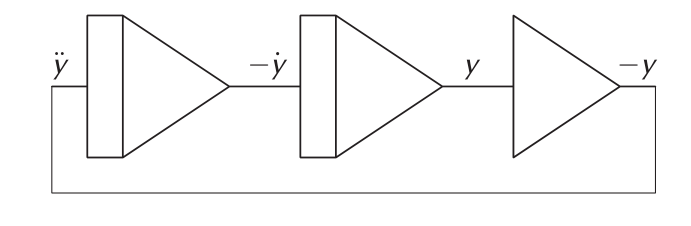
\includegraphics[width=0.6\linewidth]{../assets/analogue-computing-fun-differential-equations.png}
    \caption{Source: \url{https://chalkdustmagazine.com/features/analogue-computing-fun-differential-equations/}. (Note that this is missing initial conditions.)}
    \label{Image Label}
\end{figure}

In the above figure, the leftmost elements are the integrators, while the rightmost element is called the summer, and each elements implicitly flips the sign. Personally, there is an elegant economy to the above diagram, and furthermore, it implements such without requiring stored computer memory, and this itself is notable (as I will try to explain shortly). In contrast, implementing the same processes in digital computer architectures would require significantly more infrastructure in implementing the same mathematical laws in terms of manipulations of arbitrary symbols. Which obviously increases overall costs, size, energy requirements, and so forth.

As MacLennan wrote, in digital computation, quantities are rather arbitrary symbols that have no direct relationship to the physical systems that such may be tasked with simulating. In contrast, generally speaking, analog and physical phenomena are governed and defined by the same mathematical laws. Or as MacLennan put it, ``the computational quantities are proportional to the modeled quantities.''

With regards to latency. Imagine we somehow needed to compute one instruction for each atom, for each cell, in the human body. Which would then amount to $4 \mathrm{x} 10^{27}$ instructions.

% \begin{equation}
% \begin{split}
%     1\;\text{trillion} &= 1,000,000,000,000 = 1\,\mathrm{x}\,10^{12}\\
%     1\;\text{human} &\approx 40\;\text{trillion}\;\mathrm{cells}\\
%     1\;\text{cell} &\approx 100\;\text{trillion}\;\mathrm{atoms}
% \end{split}
% \end{equation}

To imagine this in terms of time. Consider first, simply the latency overhead incurred when your processing hardware and main memory is physically separated from each other, and therefore, each instruction must first read some datum from main memory. Lets say this overhead is $100\mathrm{ns}$ per instruction. Then latency overhead alone will amount to $4\;\mathrm{x}\;10^{20}$ seconds, or in other words, latency overhead alone will total $12,683,916,800,000$ years per evolution.

But alas, this is a ludicrous exercise for a multitude of reasons. Because, for instance, what is meant by one instruction per atom? For each evolution, can the state of each atom be computed without considering neighboring interactions? But crucially, remember the aforementioned digram that implements $\ddot{y} = -y$? Such problems needn't concern such implementations. 

\subsection*{Business Model}

The aforementioned diagram isn't ideal, on the basis that the program is essentially hardcoded or defined in the hardware configuration. Ideally, to suit the varying needs of industry, what we need are more general purpose analog computer devices. That is, they need to be programmable. 

From personal experience, there seems to be costs associated with generality, and presumably, the same extrapolates to analog devices.

Likewise, from personal experience, it seems as though technical innovation itself occurs in an incremental fashion. As though there is never some removable jump discontinuity in the graph of progress. On this grounds, working backwards, before we see whole person simulations, we will perhaps see simulations of organ groups, to individual organs, to individual cells, to individual molecular interactions within a given cell.

In the same manner, how do we define the given system that we intend to simulate? Do we begin in a bottom up fashion, and so derive quantum mechanical models of our system? Or do we begin with higher level definitions of such? In the latter, abstracting whole swaths of agents into simpler and more concise definitions, may reduce resource expenditure, but at the expense of accuracy. Presumably there exists some mean between the two tradeoffs.

For example, Sarpeshkar defined the computational environment of cells as consisting of ``highly computationally intensive nonlinear, stochastic, differential equations with $30000$ gene–protein state variables that interact via complex feedback loops.'' If our concern pertains to such a system, a top down solution would begin with a more direct model of such. While a bottom up solution would begin with the quantum mechanical physics governing such a system, which may be unnecessarily (if such is viable).

From a general perspective, we may presume that before we see computationally expensive ``bottom up'' simulations. Some mixture between the two tradeoffs will manifest, but learning more towards higher level, top down definitions of such.

Furthermore, before such evolutions may occur, each phase that manifests in the evolution of our simulation capabilities must be commercially viable, and to seed such, the initial phase in particular needs to be commercially viable. Furthermore, the beginning of such will presumably be crucial to the overall development of our industry.

Therefore, starting from the beginning. If simulating small molecules precedes simulating biochemical interactions. Then perhaps, such a business model would best begin by offering solutions to the computational chemistry and biology industry. Therein, we should note the net worth of such, which according to ``Grand View Research, Inc'', such is expected to reach $\$13.6$ billion, by 2026.\textsuperscript{(Grand View Research, Inc)}

But, we should constrain the ``Minimum Viable Product'' (MVP) to computational chemistry, presuming such to be the simplest strategy. In this regard, the utility therein is multitude. But notably at the time being: run experiments without having to first figure out how to physically synthesize the given molecules in a lab, and more generality, cheaply iterate through numerous candidates prior to cost intensive research. 

With the industry established, we may forgo full generality in our analog computer architectures, in the interest of application specific optimizations. Ideally, this also significantly simplifies supporting infrastructure. For instance, we needn't ``figure out'' how to implement general purpose analog software and programming languages.

Although a foreseeable disadvantage of an application specific software ecosystem will perhaps pertain to a smaller experienced labor pool. Furthermore, generality entails wider applicability, and so therefore, costs will likewise be further spread out from a larger consumer pool. But at the same time, if personal programming experience is applicable, it is very difficult to engineer generality in ad-hoc systems when the interactions therein isn't obvious. But very easy to do so after such systems manifests. Because we can see the interconnections and repetitions therein and -at the very least- abstract such into fewer reusable components. Therefore, if our initial viable product is successful in industry, practical generality will naturally follow.

Furthermore, specialized tools may lead to simpler tools, perhaps akin to the Elm language and it's more constrained frontend framework therein. From the business perspective, we want our customers to be deeply integrated with our products, because thereafter, changing vendors will entail costs that may not be worthwhile, since labor costs (engineers) typically exceed hardware and software expenses.

So far, we have presumed that analog computer architectures will be cheaper than the current standard of the von neumann computer architecture for the purpose of simulating natural phenomena. But how exactly is this cheaper? Currently, we cannot say, other than citing what others have speculated.


Obviously there also exists significant costs to developing and manufacturing unproven technology. But, remember when we spoke of a tradeoff between resource expenditure and accuracy? When we speak of costs, we have to consider what we are proposing in contrast to the current norm, and in this regard, if you desire accuracy, currently it's said that you're limited to simulating the effects of small molecules, on supercomputers or other high performance computing (HPC) environments where the installation and operational costs therein are significant.

Considering for instance, Tianhe-1A: initial costs amounted to $\$88$ million dollars, and another $\$20$ million dollars is spent, per year, on power consumption.\textsuperscript{(Tianhe-1)} In contrast, Trafton argues that, ``[in] one second, a [typical] cell performs about 10 million energy-consuming chemical reactions, which altogether require about one picowatt (one millionth millionth of a watt) of power.''\textsuperscript{(Trafton)} This energy efficiency therefrom, as Sarpeshkar proposes, is the product of forgoing high precision operations in favor of low precision analog computation with feedback mechanisms. Which, as Sarpeshkar argues, is fundamentally more efficient in terms of energy, time (computation) and space (memory and program installation) than digital computer architectures.

In this manner, even an approximation of the best case scenario leads to a platform that favors experimentation and iteration, by both small and underfunded terms, to billion dollar pharmaceutical companies. In a manner akin to the aforementioned software ecosystem. That is, if you can build upon abstracted systems written by experts, where these abstractions mask complexity, we may then presume that the overall barrier to entry will drop. That is again, if laypersons are able to built upon abstracted systems in a manner that doesn't require an expert understanding or formal education in such (and presumably in a manner akin to my aforementioned \url{https://imager.io} story). But on the other end, if the barrier to entry is lower, this implies reduced costs, and therefore, we may likewise see significant cost savings in industries built upon such, perhaps in a manner akin to using ``higher level'' programming languages for applicable problems. 

\section*{Engineering and Science}

The field of synthetic biology is one that attempts to unify engineering and biology. For this intersection, we have a foundation that reduces biology to software. With a proper software ecosystem in place, these bottom-up, cumulative processes may give rise to very sophisticated products, and perhaps one day, akin to the emergent phenomena seen in nature itself. Because, such an ecosystem is akin to the aforementioned ``force multiplier of the human mind''.

But perhaps too, just because software is typically easier to experiment and iterate on. You don't need a lab with specialized knowhow for the equipment, but in this case, perhaps, access to some cloud based compute infrastructure that affords easy and cheap access to the more specialized analog computing hardware. (If I happen to get into this, I'd perhaps call it SubSystems, given my \url{sub.systems} GTLD.)
